%!TEX root = ../operads_paper.tex
\section{Invertibility and group actions}
In this chapter we will investigate questions of coherence for $\Lambda$-monoidal categories with invertible objects. The goal here is to reduce these questions, whether they concern strict or weak invertible objects by \cref{L_is_K}, to the calculation of a group action. The group we will be interested in is the group of automorphisms of the unit, $L_n(I,I)$, and its action on $L_n(x,y)$ for any two objects $x$ and $y$. In \cref{splitting_as_coh}, we will explain how to use this group action to determine whether some pair of parallel morphisms in $L_n(x,y)$ are equal or not, relating this to ideas of coherence.

More intro here

\subsection{Sources and targets in \texorpdfstring{$L_n$}{L_n}}   

\begin{Defi}\label{st} For any $\ML$-monoidal category $X$, denote by $s \colon  \mathrm{Mor}(X) \rightarrow \mathrm{Ob}(X)$ and $t \colon  \mathrm{Mor}(X) \rightarrow \mathrm{Ob}(X)$ the monoid homomorphisms which send each morphism of $X$ to its source and target, respectively. That is,
  \begin{align*}
    s(f \colon  x \rightarrow y) &= x,\\
    \quad \quad t(f \colon  x \rightarrow y) &= y.
  \end{align*}
\end{Defi}

\begin{Defi}\label{s_times_t}
For a $\ML$-monoidal category $X$, define $(s \times t)(X)$ to be the pullback (in the category of monoids) $\mathrm{Ob}(X) \times_{\pi_0(X)} \mathrm{Ob}(X)$ of the diagram below. 
% \[ \begin{tikzcd}
% \mathrm{Ob}(X) \times_{\pi_0(X)} \mathrm{Ob}(X) \ar[dd, shift left=12] \ar[rr] \ar[ddrr, phantom, "\lrcorner", near start, shift left=4] & & \mathrm{Ob}(X) \ar[dd, "\lbrack \, \_ \, \rbrack"] & \\ 
% & & & \\
% \quad \quad \quad \quad \quad \quad \mathrm{Ob}(X) \ar[rr, "\lbrack \, \_ \, \rbrack"] & & \pi_0(X)
% \end{tikzcd} \]
  \[
    \xy
      (0,0)*+{\mathrm{Ob}(X) \times_{\pi_0(X)} \mathrm{Ob}(X)}="a";
      (30,0)*+{\mathrm{Ob}(X)}="b";
      (0,-20)*+{\mathrm{Ob}(X)}="c";
      (30,-20)*+{\pi_0(X)}="d";
      %
      {\ar "a" ; "b"};
      {\ar^{[\,\_\,]} "b" ; "d"};
      {\ar "a" ; "c"};
      {\ar_{[\,\_\,]} "c" ; "d"};
      %
      {\ar@{-} (2.5,-5) ; (5,-5)};
      {\ar@{-} (5,-5) ; (5,-2.5)};
    \endxy
  \]
\end{Defi}

\begin{lem}\label{stmon} Let $X$ be a $\ML$-monoidal category whose underlying category is a groupoid, and $s \times t \colon  \mathrm{Mor}(X) \rightarrow \mathrm{Ob}(X)^2$ the map induced from $s$ and $t$ using the universal property of products. Then the image of this map is $(s \times t)(X)$.
\end{lem} 


QQQ (Try to give a hint as to what we want the reader to actually recall in order to conclude this!) Recalling \cref{Gnobj,Gnconcomp,Zobj,crossconcomp}, we can immediately conclude the following.

\begin{cor} \label{stpullback}
  \[
    \begin{array}{rll} 
  		(s \times t)(\ELn) & \cong & \begin{cases}
  								\quad \mathbb{N}^{\ast n} \times_{\mathbb{N}^n} \mathbb{N}^{\ast n} & \text{if $G$ is crossed}\\
  								\quad \mathbb{N}^{\ast n} & \text{otherwise}
  							\end{cases} \\
  		& & \\
  		(s \times t)(L_n) & \cong & \begin{cases}
  								\quad \mathbb{Z}^{\ast n} \times_{\mathbb{Z}^n} \mathbb{Z}^{\ast n}  & \text{if $G$ is crossed}\\
  								\quad \mathbb{Z}^{\ast n} & \text{otherwise}
  							\end{cases} \\
    \end{array}
  \]
where the pullbacks are taken over the quotients of abelianization for $(\mathbb{N}^{\ast n})^{\ab} = \mathbb{N}^n$ and $(\mathbb{Z}^{\ast n})^{\ab} = \mathbb{Z}^n$ respectively.
\end{cor}

Before continuing further, we establish some elementary properties of the monoid $\mathbb{N}^{\ast n} \times_{\mathbb{N}^n} \mathbb{N}^{\ast n}$ and the group $\mathbb{Z}^{\ast n} \times_{\mathbb{Z}^n} \mathbb{Z}^{\ast n}$.

\begin{Defi}\label{length}
Let $S$ be a set, and consider the free monoid $\N^{*S}$ given by words in the elements of $S$. \emph{Length} $\ell \colon \N^{*S} \rightarrow \N$ is the monoid homomorphism which is given by the identity homomorphism on each copy of $\N$ in the coproduct $\N^{*S}$. Concretely, the length $\ell(w)$ of a word $w \in \N^{*S}$ is the total number of letters in it.
\end{Defi}

Shortly we will show that $\mathbb{N}^{\ast n} \times_{\mathbb{N}^n} \mathbb{N}^{\ast n}$ is a free monoid. In order to do this we will describe a set of elements which act as the generators for this free monoid. But before this we describe some properties of elements in the pullback $\mathbb{N}^{\ast n} \times_{\mathbb{N}^n} \mathbb{N}^{\ast n}$. 

First, let $a_1$, $\ldots$, $a_n$ be the generators for the first copy of $\mathbb{N}^{\ast n}$ in $\mathbb{N}^{\ast n} \times_{\mathbb{N}^n} \mathbb{N}^{\ast n}$, and let $x_1$, $\ldots$, $x_n$ be the generators for the second copy of $\mathbb{N}^{\ast n}$. A typical element of $\mathbb{N}^{\ast n} \times_{\mathbb{N}^n} \mathbb{N}^{\ast n}$ can be written uniquely using these generators as
  \[
    (w,w') = \left(a_{i_1}a_{i_2}\cdots a_{i_k}, x_{j_1}x_{j_2}\cdots x_{j_l}\right)
  \]
and, since this is an element of the pullback, we know that $k = l$. I.e., $l(w) = l(w')$. A good thing to keep in mind here is that since the pullback is taken over the `connected components' morphism then each of $w$ and $w'$ must feature the same number of instances of each index for the generators $a_i$ and $x_j$. For example, $\left(x_2 x_1 x_2, a_1 a_1 a_2\right)$ is not an element of $\mathbb{N}^{\ast 2} \times_{\mathbb{N}^2} \mathbb{N}^{\ast 2}$, but $\left(x_2 x_1 x_2, a_2 a_2 a_1\right) \emph{is}$.

\begin{Defi}\label{indecomposable}
An element $\left(a_{i_1}a_{i_2}\cdots a_{i_k}, x_{j_1}x_{j_2}\cdots x_{j_k}\right) \in \mathbb{N}^{\ast n} \times_{\mathbb{N}^n} \mathbb{N}^{\ast n}$ to be \emph{indecomposable} if there does not exist $h < k$ such that $\left(a_{i_1}a_{i_2}\cdots a_{i_h}, x_{j_1}x_{j_2}\cdots x_{j_h}\right)$ is also an element of $\mathbb{N}^{\ast n} \times_{\mathbb{N}^n} \mathbb{N}^{\ast n}$. 
\end{Defi}

As an example to help explain the previous definition, the element $(a_2 a_1, x_2 x_1)$ is \emph{not} an indecomposable element of $\mathbb{N}^{\ast 2} \times_{\mathbb{N}^2} \mathbb{N}^{\ast 2}$ since $(a_2, x_2) \in \mathbb{N}^{\ast 2} \times_{\mathbb{N}^2} \mathbb{N}^{\ast 2}$. However, $(a_2 a_1, x_1 x_2)$ \emph{is} an indecomposable element of $\mathbb{N}^{\ast 2} \times_{\mathbb{N}^2} \mathbb{N}^{\ast 2}$ since $(a_2, x_1) \notin \mathbb{N}^{\ast 2} \times_{\mathbb{N}^2} \mathbb{N}^{\ast 2}$, due to the mismatch in the number of instances of each index.

It is fairly clear how to express each element as a product of indecomposables --- in essence, we keep splitting the element until we can't split it any further. For example, consider the element $\left(a_3 a_1 a_2 a_2 a_1 a_3, x_2 x_1 x_3 x_2 x_3 x_1\right) \in \mathbb{N}^{\ast 3} \times_{\mathbb{N}^3} \mathbb{N}^{\ast 3}$. We can write this as
  \begin{align*}
    \left(a_3 a_1 a_2 a_2 a_1 a_3, x_2 x_1 x_3 x_2 x_3 x_1\right) &= \left(a_3 a_1 a_2 a_2, x_2 x_1 x_3 x_2\right)\left(a_1 a_3, x_3 x_1\right) \\
    &= \left(a_3 a_1 a_2, x_2 x_1 x_3\right)\left(a_2, x_2\right)\left(a_1 a_3, x_3 x_1\right).
  \end{align*}
We will make use of this idea of splitting elements into indecomposable elements in the following proof.

\begin{lem}\label{freemon} $\mathbb{N}^{\ast n} \times_{\mathbb{N}^n} \mathbb{N}^{\ast n}$ is a free monoid generated by the indecomposable elements.
\end{lem}
\begin{proof}
We will show how each element of $\mathbb{N}^{\ast n} \times_{\mathbb{N}^n} \mathbb{N}^{\ast n}$ can be written uniquely as a product of the indecomposable elements. We have already described how each element is a product of indecomposables. We show here that each such product is unique. For suppose that $(w, w') = \left(a_{i_1}a_{i_2} \cdots a_{i_k}, x_{j_1} x_{j_2} \cdots x_{j_k}\right)$ could be written as a product of indecomposables in two different ways, say
  \[
    (w,w') = c_1 c_2 \cdots c_s = d_1 d_2 \cdots d_t.
  \]
Then the length of $c_1$ must either be strictly less than or strictly greater than the length of $d_1$; if they had equal length, then they would be equal. Without loss of generality, assume that $l(c_1) < l(d_1)$. Then the first $l(c_1)$ terms appearing in $d_1$ would agree with $c_1$, since $c_1$ is indecomposable, hence $d_1 = c_1 d_1'$, where $d_i$ is another, possibly indecomposable, element of $\mathbb{N}^{\ast n} \times_{\mathbb{N}^n} \mathbb{N}^{\ast n}$. Hence, $d_1$ is not indecomposable.

The proof can be finished using a straightforward induction argument on the number of terms in $(w,w')$. We would start by comparing $c_1$ and $d_1$, as above, before `cancelling' any common terms on the left of the words and proceeding with the same argument as before. For example, where $l(c_1) < l(d_1)$ we would find that $d_1 = c_1 d_1'$ and so go on to consider $c_2 c_3 \cdots c_s = d_1' d_2 \cdots d_t$. Since the argument begins with all terms being indecomposable, we would first split $d_1'$ into a product of indecomposables. The induction then follows to show that $\mathbb{N}^{\ast n} \times_{\mathbb{N}^n} \mathbb{N}^{\ast n}$ is freely generated on the set of indecomposable elements.

QQQ Consider the universal property argument instead for the last bit. It may make the argument slicker and less woolly at the end.
QQQ (New proof above, old proof below)

Write the generators for the first copy of $\mathbb{N}^{\ast n}$ in $\mathbb{N}^{\ast n} \times_{\mathbb{N}^n} \mathbb{N}^{\ast n}$ as $a_1, \ldots, a_n$, and the generators for the second copy of $\mathbb{N}^{\ast n}$ as $x_1, \ldots, x_n$. An element $(w,w') \in \mathbb{N}^{\ast n} \times_{\mathbb{N}^n} \mathbb{N}^{\ast n}$ can therefore be written uniquely as
  \[
    (w,w') = (a_{i_1} a_{i_2} \cdots a_{i_k}, x_{i_1} x_{i_2} \cdots x_{i_j}),
  \]
which, being an element of the pullback, immediately implies $k=j$. We then define an element $ (a_{i_1} a_{i_2} \cdots a_{i_k}, x_{i_1} x_{i_2} \cdots x_{i_k})$ of $\mathbb{N}^{\ast n} \times_{\mathbb{N}^n} \mathbb{N}^{\ast n}$ to be indecomposable if there does not exist an $h < k$ such that $ (a_{i_1} a_{i_2} \cdots a_{i_h}, x_{i_1} x_{i_2} \cdots x_{i_h})$ is also an element of $\mathbb{N}^{\ast n} \times_{\mathbb{N}^n} \mathbb{N}^{\ast n}$. It is clear that every element can be written as a product of indecomposables.

If $(w,w')$ can be written as a product of indecomposables in two ways, say 
  \[
    (w,w') = c_1 \cdots c_s = d_1 \cdots d_t,
  \]
then the length  of $c_1$ must be either strictly less than or strictly greater than the length of $d_1$; if they had equal length, then they would be equal. Without loss of generality assume $\ell(c_1) < \ell(d_1)$. But then the first $\ell(c_1)$ terms appearing in $d_1$ would agree with $c_1$, proving that $d_1$ is not indecomposable. Straightforward induction then finishes the proof that every element of $\mathbb{N}^{\ast n} \times_{\mathbb{N}^n} \mathbb{N}^{\ast n}$ can be written as a product of indecomposables in a unique way, making $\mathbb{N}^{\ast n} \times_{\mathbb{N}^n} \mathbb{N}^{\ast n}$ free on the set of indecomposables.
\end{proof}

Recall the $\ML$-monoidal functors $\delta \colon \ELnn \rightarrow \ELnn$ and $q \colon \ELnn \rightarrow L_n$. The construction $X \mapsto (s \times t)(X)$ is a functor $\lmc \rightarrow \mon$, so these induce monoid homomorphisms that we also write, by abuse of notation, as 
  \begin{align*}
    (\delta, \delta) \colon  \mathbb{N}^{\ast 2n} \times_{\mathbb{N}^{2n}} \mathbb{N}^{\ast 2n} &\rightarrow \mathbb{N}^{\ast 2n} \times_{\mathbb{N}^{2n}} \mathbb{N}^{\ast 2n}, \\
    (q, q) \colon  \mathbb{N}^{\ast 2n} \times_{\mathbb{N}^{2n}} \mathbb{N}^{\ast 2n} &\rightarrow \mathbb{Z}^{\ast n} \times_{\mathbb{Z}^n} \mathbb{Z}^{\ast n}. 
  \end{align*}

\begin{lem}\label{monoid_coeq}
The monoid homomorphism $(q,q)$ exhibits $\mathbb{Z}^{\ast n} \times_{\mathbb{Z}^n} \mathbb{Z}^{\ast n}$ as the cokernel of the monoid homomorphism $(\delta, \delta)$.
\end{lem}
\begin{proof}
QQQ I'm not sure this is correct, or if it is then it isn't obvious as claimed.
\end{proof}

\begin{lem}\label{rho_lemmas}
If $(w,w') \in \mathbb{N}^{\ast 2n} \times_{\mathbb{N}^{2n}} \mathbb{N}^{\ast 2n}$ is indecomposable, then so is $\delta(w,w')$. For any indecomposable $(w,w')$, there exists a unique natural number $k$ and indecomposable $(v,v')$ such that
  \[
    (w,w') = \delta^k(v,v')
  \]
but $(v,v')$ is not $\delta(u,u')$ for any indecomposable $(u,u')$.
\end{lem}
\begin{proof}
The first statement follows immediately from the injectivity of $\delta$ on objects, and the second from the fact that $\delta$ doubles the length of any element.
\end{proof}


We now want to show that the group $(s \times t)(L_n)$ we have described is in fact a submonoid of $\MorLn$. We will accomplish this  by first proving the analogous statement for all $\ELn$. For any pair $(w, w') \in \mathbb{N}^{\ast n} \times_{\mathbb{N}^n} \mathbb{N}^{\ast n}$ such that the images of $w$ and $w'$ in the commutative monoid $\mathbb{N}^n$ are the same, there are generators $x_1, \ldots, x_m$ for which 
  \[
    w = x_1 \otimes \ldots \otimes x_m
  \]
and there exists at least one permutation $\sigma \in \Sigma_m$ such that
  \[
    w' = x_{\sigma(1)} \otimes \ldots \otimes x_{\sigma(m)}.
  \]
Since the underlying permutation maps $\pi \colon \Lambda(m) \rightarrow \Sigma_m$ of a crossed action operad $\ML$ are all surjective, we can always find an element of $g \in \Lambda(m)$ for which $\pi(g) = \sigma$. 

\begin{nota}\label{rho_ww'}
Let $\rho \colon \mathbb{N}^{\ast n} \times_{\mathbb{N}^n} \mathbb{N}^{\ast n} \rightarrow \Lambda^{\oplus}$ be an arbitrary, but fixed, function such that $\rho(w,w')$ satisfies $\pi(\rho(w,w')) = \sigma$ as defined above.
\end{nota}

We can now construct the desired injection using the function $\rho$ from \cref{rho_ww'}.
\begin{prop}\label{stGnsub} $\mathrm{Mor}(\ELn) \rightarrow (s \times t)(\ELn)$ is a split epi of monoids, so $(s \times t)(\ELn)$ is (isomorphic to) a submonoid of $\mathrm{Mor}(\ELn)$. Furthermore, we can choose the injection $i \colon (s \times t)(\ELn) \rightarrow \mathrm{Mor}(\ELn)$ such that the following diagram commutes.
\begin{center}
    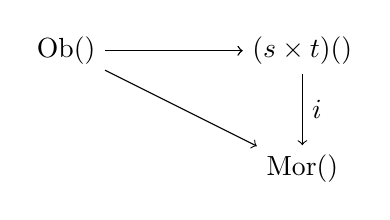
\begin{tikzpicture}[x=30mm,y=15mm]
		\node (a) at (0,0) {$\mathrm{Ob}(\ELn)$};
		\node (b) at (1,0) {$(s \times t)(\ELn)$};
		\node (d) at (1,-1) {$\mathrm{Mor}(\ELn)$};
      \draw [->] (a) to (b);
			\draw [->] (a) to node [above] {$$} (b);
			\draw [->] (b) to node [right] {$i$} (d);
			\draw [->] (a) to node [below,left] {$$} (d);
    \end{tikzpicture}
\end{center}		
\end{prop}
\begin{proof}
First, assume that the action operad $\ML$ is not crossed. Then there exists an injective monoid homomorphism
% \[ \begin{array}{rlrll}
% 			i & \colon & (s \times t)(\ELn) & \rightarrow & \mathrm{Mor}(\ELn) \\
% 			& \colon & \mathbb{N}^{\ast n} & \rightarrow & \lop \times_{\mathbb{N}} \mathbb{N}^{\ast n} \\
% 			& \colon & w & \mapsto & ( \, e_{|w|}, w \, ),
% 		\end{array}
% \]
  \begin{align*}
    i \colon (s \times t)(\ELn) &\rightarrow \mathrm{Mor}(\ELn) \\
    w & \mapsto (e_{|w|}, w)
  \end{align*}
which is clearly seen when considering $i$ as a homomorphism $\mathbb{N}^{\ast n} \rightarrow \lop \times_{\mathbb{N}} \mathbb{N}^{\ast n} $ and where we have written $e_{|w|}$ for the identity in the group $\Lambda(|w|)$. The homomorphism property follows from the fact that the length $|w|$ defined in \cref{lengthdef} is itself a homomorphism, so $|w \oplus w'| = |w|+|w'|$. Thus $(s \times t)(\ELn) \subseteq \mathrm{Mor}(\ELn)$ for non-crossed $\ML$, and the splitting is obvious.

Now assume that $\ML$ is crossed. Fix a function $\rho$ as in \cref{rho_ww'}. Since $\mathbb{N}^{\ast n} \times_{\mathbb{N}^n} \mathbb{N}^{\ast n}$ is a free monoid  by \cref{freemon}, there exists a unique monoid homomorphism
  \[
    \rho \colon \mathbb{N}^{\ast n} \times_{\mathbb{N}^n} \mathbb{N}^{\ast n} \longrightarrow \lop
  \]
which agrees with the original function $\rho$ on the generators in the source. By construction,
  \[
    \pi(\rho(w, w'))(w) = w'
  \]
for any $(w, w') \in\mathbb{N}^{\ast n} \times_{\mathbb{N}^n} \mathbb{N}^{\ast n}$, not just the generators. Using $\rho$ we define the homomorphism $i$ to be as follows.
  \begin{align*}
		i \colon (s \times t)(\ELn) &\rightarrow \mathrm{Mor}(\ELn) \\
		\mathbb{N}^{\ast n} \times_{\mathbb{N}^n} \mathbb{N}^{\ast n} &\rightarrow \lop \times_{\mathbb{N}} \mathbb{N}^{\ast n} \\
		(w, w') &\mapsto ( \, \rho(w, w'), w \, )
	\end{align*}
Moreover, for any two elements $(v, v')$, $(w, w')$ of $\mathbb{N}^{\ast n} \times_{\mathbb{N}^n} \mathbb{N}^{\ast n}$ we find that if
  \[
    i(v,v') = (\rho(v,v'),v) = (\rho(w,w'),w) = i(w,w'),
  \]
then $\rho(v,v') = \rho(w,w')$ and $v = w$. So then
  \[
    v' = \pi(\rho(v,v'))(v) = \pi(\rho(w,w'))(w) = w',
  \]
hence $i$ is injective. This injection splits $\mathrm{Mor}(\ELn) \rightarrow (s \times t)(\ELn)$ by construction.

For the final statement, note that the inclusion of $\mathrm{Ob}(\ELn)$ into $(s \times t)(\ELn)$ sends an object $w$ to the pair $(w,w)$. The only indecomposable such are $(x_i, x_i)$ if we write the generating objects of $\ELn$ as $x_1, x_2, \ldots, x_n$. Using the construction above, we can always choose $\rho(x_i, x_i) = e_1$.
\end{proof}

For the proof of \cref{stGnsub}, $\rho$ can be any function satisfying the criteria in \cref{rho_ww'}, with the caveat that commuting with the inclusion of objects requires $\rho(x_i, x_i) = e_1$. The analogous proof for $L_n$, though, requires more properties of $\rho$ which we establish now. Recall the functor $\delta$ from \cref{qdef}. Note that by construction it restricts to a monoid homomorphism on sets of objects, and we denote this restriction by $\delta$ as well in the lemma below.

\begin{prop} \label{stZsub} $\MorLn \rightarrow (s \times t)(L_n)$ is a split epi of monoids, so $(s \times t)(L_n)$ is (isomorphic to) a submonoid of $\MorLn$. Furthermore, we can choose the injection $i \colon (s \times t)(L_n) \rightarrow \MorLn$ such that the following diagram commutes.
\begin{center}
    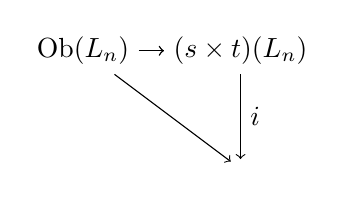
\begin{tikzpicture}[x=20mm,y=15mm]
		\node (a) at (0,0) {$\mathrm{Ob}(L_n)$};
		\node (b) at (1,0) {$(s \times t)(L_n)$};
		\node (d) at (1,-1) {$\MorLn$};
      \draw [->] (a) to (b);
			\draw [->] (a) to node [above] {$$} (b);
			\draw [->] (b) to node [right] {$i$} (d);
			\draw [->] (a) to node [below,left] {$$} (d);
    \end{tikzpicture}
\end{center}		
\end{prop}
\begin{proof}
Let $i \colon (s \times t)(\ELnn) \rightarrow \mathrm{Mor}(\ELnn)$ be a splitting as in \cref{stGnsub}. We will first show that the function $\rho$ can be chosen to make the square
\begin{center}
    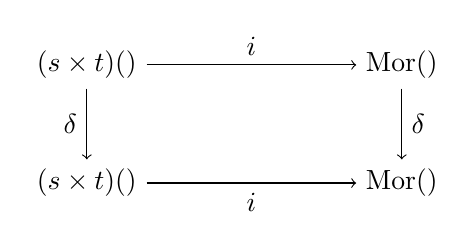
\begin{tikzpicture}[x=20mm,y=15mm]
		\node (a) at (0,0) {$(s \times t)(\ELnn)$};
		\node (b) at (2,0) {$\mathrm{Mor}(\ELnn)$};
		\node (c) at (0,-1) {$(s \times t)(\ELnn) $};
		\node (d) at (2,-1) {$\mathrm{Mor}(\ELnn)$};
			\draw [->] (a) to node [above] {$i$} (b);
			\draw [->] (b) to node [right] {$\delta$} (d);
			\draw [->] (a) to node [left] {$\delta$} (c);
			\draw [->] (c) to node [below] {$i$} (d);
    \end{tikzpicture}
\end{center}
commute. Recall that $i$ is defined by first factoring an element into indecomposables, and then applying $\rho$ to each of those. Thus on an indecomposable $(w,w')$, the commutativity of this square is the claim that $\delta(\rho(w,w')) = \rho(\delta w, \delta w')$ using that $\delta(w,w') = (\delta w, \delta w')$ is also indecomposable by the first part of \cref{rho_lemmas}. By the second part of \cref{rho_lemmas}, write $(w,w') = \delta^k(v,v')$ for a unique $(v, v')$ which is not in the image of $\delta$, so the equation $\delta(\rho(w,w')) = \rho(\delta w, \delta w')$ is equivalent to
  \[
    \delta\left(\rho\left(\delta^k(v,v')\right)\right) = \delta^{k+1}\rho(v,v').
  \]
Furthermore, $(v,v')$ cannot be written as $\delta(u,u')$ for any indecomposable $(u,u')$, so we may choose $\rho(v,v')$ arbitrarily and this will uniquely determine $i$ in such a way that the square commutes. 

The functor $q \colon \ELnn \rightarrow L_n$ is the cokernel of $\delta$, so the composite
  \[
    \mathrm{Mor}(\ELnn) \stackrel{\mathrm{Mor}\delta}{\longrightarrow} \mathrm{Mor}(\ELnn) \stackrel{\mathrm{Mor}q}{\longrightarrow} \MorLn
  \]
is the zero map. From the definition of $\delta$ in \cref{qdef} and the description of the monoids $(s \times t)(\ELn), (s \times t)(L_n)$ in \cref{stpullback}, the composite
  \[
    (s \times t)(\ELnn) \stackrel{(s \times t)(\delta)}{\longrightarrow}  (s \times t)(\ELnn) \stackrel{(s \times t)(q)}{\longrightarrow} (s \times t)(L_n)
  \]
exhibits $(s \times t)(L_n)$ as the cokernel of $(s \times t)(\delta)$ QQQ this is \cref{monoid_coeq} QQQ so induces a unique monoid homomorphism $i \colon  (s \times t)(L_n) \rightarrow \MorLn$ making the square below commute.
\begin{center}
    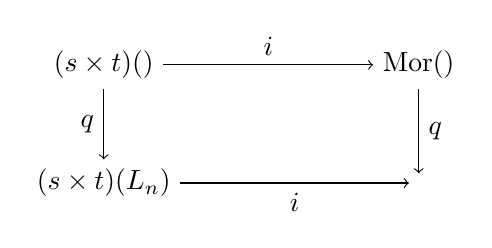
\begin{tikzpicture}[x=20mm,y=15mm]
		\node (a) at (0,0) {$(s \times t)(\ELnn)$};
		\node (b) at (2,0) {$\mathrm{Mor}(\ELnn)$};
		\node (c) at (0,-1) {$(s \times t)(L_n) $};
		\node (d) at (2,-1) {$\MorLn$};
			\draw [->] (a) to node [above] {$i$} (b);
			\draw [->] (b) to node [right] {$q$} (d);
			\draw [->] (a) to node [left] {$q$} (c);
			\draw [->] (c) to node [below] {$i$} (d);
    \end{tikzpicture}
\end{center}
This homomorphism $i$ splits $\MorLn \rightarrow (s \times t)(L_n)$ as desired.

QQQ (Check this properly, might need a bit more to say this is true.) The final claim about commuting with the inclusion of objects follows using the same argument as in  \cref{stGnsub}, so we must also require $\rho(x_i, x_i) = e_1$.

\end{proof} 

\subsection{Unit endomorphisms of \texorpdfstring{$L_n$}{L_n}}

We now consider the monoid of unit endomorphisms, $L_n(I,I)$. This is a particularly important submonoid of the morphisms $\MorLn$, since it is the only submonoid which is also a homset of the category $L_n$. Moreover, because the maps in $L_n(I,I)$ all share the same source and target, what we have is not just a monoid under tensor product but also under composition as well. This fact leads to a series of special properties for $L_n(I,I)$, the first of which is just another instance of the classic Eckmann-Hilton argument. 

\begin{prop} \label{endcom} $L_n(I,I)$ is a commutative monoid under both tensor product and composition, with $f \otimes f' = f \circ f'$. Since $L_n$ is a groupoid, this commutative monoid is actually an abelian group.
\end{prop}

In fact, we have the following corollary of \cref{tensinv_basic} in the case that $X = L_n$.

\begin{cor} \label{tensinv} Every morphism $f \colon  w \rightarrow v$ in $L_n$ has an inverse under tensor product, $f^* \colon  w^* \rightarrow v^*$. That is, the monoid $\MorLn$ is actually a group and $L_n(I,I)$ is a subgroup.
\end{cor}



\begin{prop} \label{endnorm} $L_n(I,I)$ is a normal subgroup of $\MorLn$. Moreover, if $\ML$ is a crossed action operad, then $L_n(I,I)$ is a subgroup of the center of $\MorLn$.
\end{prop}
\begin{proof}
From \cref{tensinv}, we know that $L_n(I,I)$ is a subgroup of $\MorLn$. For normality, we need to again consider both crossed and non-crossed cases separately. 

If $\ML$ is not crossed, then by \cref{crossconcomp} we know that the map assigning objects of $L_n$ to their connected component is just the identity $\id_{\mathbb{Z}^{\ast n}}$. In other words, every object belongs to its own unique component, so that every morphism of $L_n$ is actually an endomorphism. It follows that the group $L_n(I,I)$ is the kernel of the source homomorphism $s$ from \cref{st} and thus normal.

For crossed $\ML$, recall from \cref{spacial} that all $\ML$-monoidal categories are spacial, and so in particular $L_n$ is. This means that for any $h \in L_n(I,I)$ and $w \in \mathrm{Ob}(L_n)$ we will always have $h \otimes w = w \otimes h$. Thus for any $f \colon w \rightarrow v$ in $\MorLn$, we find that
  \begin{align*}
  	h \otimes f & =(\id_I \circ h) \otimes (f \circ \id_w) \\
  	&= (I \otimes f) \circ (h \otimes w) \\
  	&= (f \otimes I) \circ (w \otimes h) \\
  	&= (f \circ \id_w) \otimes (\id_I \circ h) \\
  	&= f \otimes h
  \end{align*}
and so $L_n(I,I)$ is a subgroup of the center of $\MorLn$, thus normal. 
\end{proof}

\subsection{Splitting the monoid of morphisms}

In this section we will collect together many of the arguments of this chapter to give the first closed form expression for the automorphism group of the unit object, $I$, in $L_n$.
\begin{prop}\label{morprod} For any action operad $\ML$,
  \[
    \MorLn \cong (s \times t)(L_n) \ltimes L_n(I,I).
  \]
Moreover, if $\ML$ is a crossed action operad, then
  \[
    \MorLn \cong (s \times t)(L_n) \times L_n(I,I).
  \]
\end{prop}
\begin{proof}
We just saw in \cref{endnorm} that $L_n(I,I)$ is a normal subgroup of $\MorLn$, so we can consider the quotient group
% \[ \begin{tikzcd}
% L_n(I,I) \ar[r, hookrightarrow] & \MorLn \ar[r] & \bigquotient{\MorLn}{L_n(I,I)}
% \end{tikzcd} \]
\[
  L_n(I,I) \hookrightarrow \MorLn \rightarrow \bigquotient{\MorLn}{L_n(I,I)}
\]
By the universal property of quotients, the map $\MorLn \rightarrow \MorLn / L_n(I,I)$ will uniquely factor any homomorphism whose composite with the inclusion $L_n(I,I) \hookrightarrow \MorLn$ is the zero map. But our source/target map $s \times t \colon \MorLn \rightarrow (s \times t)(L_n)$ is one such homomorphism, since for any $h \colon  I \rightarrow I$ we find that $(s \times t)(h) = (I, I)$, which is the identity element in $(s \times t)(L_n)$. Therefore there must exist a unique homomorphism $u$ making the triangle below commute:
% \[ \begin{tikzcd}
% \MorLn \ar[dd] \ar[ddrr, "s \times t"] & & \\
% & & \\
% \bigquotient{\MorLn}{L_n(I,I)} \ar[rr, "u"] & & (s \times t)(L_n)
% \end{tikzcd} \]
  \[
    \xy
      (0,0)*+{\MorLn}="a";
      (0,-20)*+{\bigquotient{\MorLn}{L_n(I,I)}}="b";
      (40,-20)*+{(s \times t)(L_n)}="c";
      %
      {\ar "a" ; "b"};
      {\ar^{s \times t} "a" ; "c"};
      {\ar_{u} "b" ; "c"};
    \endxy
  \]
This map $u$ will be surjective --- since $s \times t$ is --- but in fact it is also injective. This is because if two morphisms $f$, $f'$ of $L_n$ have the same source and target, then the map $h = f^* \otimes f'$ is an element of $L_n(I,I)$ for which $f \otimes h = f'$, and so $f$ and $f'$ are part of the same equivalence class in $\MorLn/L_n(I,I)$. 

Thus $u$ is bijective, so that
  \[
    \bigquotient{\MorLn}{L_n(I,I)} \cong (s \times t)(L_n)
  \]
and there is a group extension
% \[ \begin{tikzcd}
% 0 \ar[r] & L_n(I,I) \ar[r, hookrightarrow] & \MorLn \ar[r, "s \times t"] & (s \times t)(L_n) \ar[r] & 0.
% \end{tikzcd} \]
  \[
    0 \rightarrow L_n(I,I) \hookrightarrow \MorLn \xrightarrow{(s \times t)} (s \times t)(L_n) \rightarrow 0.
  \]
But recall from \cref{stZsub} that this extension is split, or equivalently $\MorLn$ is a semi-direct product $(s \times t)(L_n) \ltimes L_n(I,I)$. However, if $G$ is crossed then we also saw in \cref{endnorm} that $L_n(I,I)$ is a subgroup of the center of $\MorLn$, and so it will follow that $\MorLn$ is also a central extension of $(s \times t)(L_n)$. In that case $\MorLn$ is just the direct product $(s \times t)(L_n) \times L_n(I,I)$.
\end{proof}

\begin{cor}\label{lnII_mormodst}
If $\ML$ is crossed, then $L_n(I,I) \cong \MorLn / (s \times t)(L_n)$.
\end{cor}

\begin{conv}
In what follows (in particular, \cref{conseq_spl,full_des}), we fix an isomorphism $\MorLn \cong (s \times t)(L_n) \times L_n(I,I)$; we note that this isomorphism (and in particular the projection homomorphism $\MorLn \rightarrow L_n(I,I)$) depends on the choices made in the proof of \cref{stZsub}.

\end{conv}

\subsection{Splitting as a coherence theorem}\label{splitting_as_coh}

Coherence theorems often take the form of a statement that all diagrams with a certain property commute. For example, coherence for ordinary monoidal categories states that every diagram in the free monoidal category generated by a set of objects commutes and coherence for symmetric monoidal categories states that a pair of parallel morphisms (i.e., the two legs around some diagram of interest) are equal if and only if their underlying permutations are equal.

\begin{thm}\label{split_coh}
Let $\ML$ be an action operad, and $L_n$ the free $\ML$-monoidal category on $n$ invertible objects. Let $x, y$ be objects of $L_n$, and $f, g \colon  x \rightarrow y$ morphisms between them. Then the following are equivalent:
\begin{enumerate}
\item $f = g$,
\item $g^{-1} f = \id_x$, and
\item the automorphism of the unit object $x^{-1} \otimes \left(g^{-1} f\right)$ is the identity in $L_n(I,I)$.
\end{enumerate}
\end{thm}
\begin{proof}
(1) implies (2) and (2) implies (3) are trivial. For (3) implies (1), we need only note that the invertibility of $x$ means that the function $x \otimes - \colon L_n(I,I) \rightarrow L_n(x,x)$ is a monoid isomorphism (with inverse $x^{-1} \otimes -$) so sends identities to identities.
\end{proof}

In practice, computing $x^{-1} \otimes \left(g^{-1} f\right)$ from $g^{-1} f$ is relatively simple, so we should view this theorem as affording the following strategy for resolving the potential equality of a pair of parallel morphisms $f, g \colon x \rightarrow y$.
\begin{enumerate}
\item Determine the group $L_n(I,I)$ in such a way as to make the equality of two elements computable in a practical fashion.
\item Compute $x^{-1} \otimes \left(g^{-1} f\right)$ as an element of this group.
\end{enumerate}
The following chapters are devoted to the first step of this strategy.
